\section{Results}
\label{sec:rslts}

%introduction

\subsection{Clustering Results}
\label{ssec:clures}
\mynote[author=Harrie]{Je verhaal is moeilijk te volgen omdat de resultaten die je bespreekt in de appendix staat, zet de belangrijke resultaten in de text. (Hyperparameters horen wel in de appendix.)}
In this part the results of the clustering of both the user and job features is described.
The first attempt is to cluster the user or job data using the K-prototypes algorithm which can deal with both numerical and categorical data.
To improve the clustering results the numerical data is converted to \textit{z}-scores.
When this algorithm is applied the clustering time after time breaks down around cluster size 50. If after this point the number of clusters is increased the algorithm fails to initiate the cluster centroids.
Various cluster initiation schemes and even manual initiation have been tried, but the problem persists.

Due to the fact that the K-prototypes could not be used and because of the fact that only a few columns were numerical it was decided to treat all numerical data as categorical data and to apply the K-modes algorithm.
For the users the optimal cluster size seems to be around 150 and for jobs around 100 (figure \ref{fig:eb})
However, the elbow plots do not show a determinative point where they flatten out.
Thus to validate the clustering results the cluster sizes 25 till 300 with an interval of 25 were tested on 12 scenarios for both Logistic Regression and Neural Network.
In total 288 tests were conducted (12 different cluster size $\times$ 12 scenarios $\times$ 2 algorithms). 
The table of the best results can be found in appendix \ref{ssec:cluscen}.
The results do not show any improvement over the baseline, and therefore it can be concluded that the clustering cannot be applied for the recommender system.

\begin{figure}[H]
    \centering
    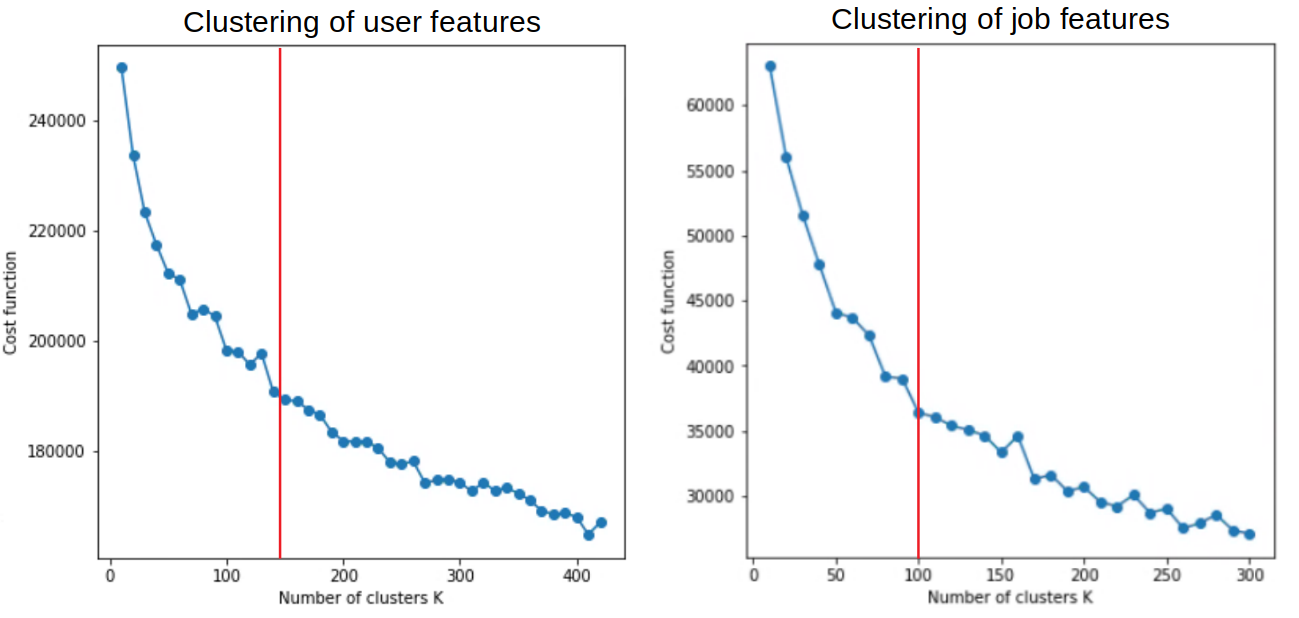
\includegraphics[width=\linewidth]{ThesisTemplate/Images/Clustering.png}
    \caption{\label{fig:eb} \footnotesize{Elbow Plots Users and Jobs Clustering}}
\end{figure}

As second method it is attempted to spread the Term Frequency-Inverse Document Frequency scores (TF-IDF) of the job descriptions over meaningful clusters.
Plotting the scores in an Elbow plot (appendix \ref{ssec:Kmeans}) does not show a point where the line flats out.
Visual inspection comparing the clusters with the related job title displayed randomness.
The job descriptions contain a great diversity of words, while the observations (8,265) is relatively low.
It can be argued that this technique can yield better results if the number of observations is higher. 
Therefore, for this research it was decided to not further pursue this approach.

The third clustering approach is to cluster the n-grams of the job title characters. 
The job titles are distributed over 286 clusters, and although through a visual inspection comparing the assigned clusters with the associated job titles the clustering seems to deliver good results, when looking at the metrics the performance is worse than the K-modes clustering.
The hierarchical clustering results can be found in appendix \ref{ssec:hieclu}.

The job data contains a number of recurring job titles that are exactly the same, and based on the hierarchical clustering results it can be assumed that even though the job title is the same the underlying features deviate. 
To verify this assumption the cosine similarities of a job vector versus all other job vectors for all observations was calculated.
None of the returned similarities give an exact match, so highly similar job vectors can have very different associated job titles.
Therefore it can be reasoned that although job titles sometimes are the exact same or very similar the underlying features are different.


% \begin{table}[h]
% \begin{footnotesize}
% \begin{tabular}{llll}
\toprule
\textbf{Scenario}   & \textbf{\# clusters}  & \textbf{Accuracy} & \textbf{MCC}    \\
\midrule
1                   & 225                   & 0.81              & 0.41            \\ %6.7
2                   & 275                   & 0.82              & 0.49            \\ %6.15
3                   & 300                   & 0.75              & 0.08            \\ %6.8
4                   & 100                   & 0.77              & 0.05            \\ %6.13
5                   & 225                   & 0.82              & 0.45            \\ %6.2
6                   & 300                   & 0.77              & 0.27            \\ %6.3
7                   & 250                   & 0.84              & 0.55            \\ %6.14 
9                   & 150                   & 0.79              & 0.27            \\ %6.12
10                  & 25                    & 0.15              & 0.11            \\ %6.4
11                  & 25                    & 0.93              & 0.92            \\ %6.6
12                  & 25                    & 0.11              & 0.05            \\ %6.10 
13                  & 25                    & 0.89              & 0.88            \\ %6.11
\bottomrule
\end{tabular}
% \end{footnotesize}
% \caption{\label{tab:clures} Best Results Clustering}
% \end{table}

\subsection{Results Content-Based Learning Models}
\mynote[author=Harrie]{Een confusion matrix zou hier heel goed werken, of anders iets van (percentage) false/true positives/negatives, omdate de MCC toch moeilijk te interpreteren is.}
When assessing the accuracy results it must be taken into account that the dataset exhibits a class imbalance of 79\% being positive labels and 21\% being negative labels.
The consequence of this imbalance is that if the classifier predicts all labels to be positive it achieves 0.79 accuracy.
This fallaciously suggests that the classification results are decent.
Here is where the utility of the Matthews correlation coefficient (MCC) comes into play, as the MCC in such case will be 0.00 because no labels are classified as negative.

The classification results of the models are shown in table \ref{tab:res}.
Judging only on the accuracy alone it does not seem to make a great difference which model is applied.
When the MCC scores are analyzed the Neural Network performs 10\% better than its closest rival and 52\% better than the baseline.
The higher performance of MCC suggests better balanced predictions of both the positive and negative labels.
The best scores for the Neural Network were achieved with a setup of one hidden layer.
When more hidden layers are added the performance decays gradually.
The more hidden layers the more complex patterns the Neural Network can learn, on the other hand this also increases the chance of overspecialization (overfitting) on the train data.
Therefore, it can be argued that when extra layers are added the performance is worsened due to overfitting.

\begin{table}[h]
\begin{footnotesize}
\begin{tabular}{lrr}
\toprule
\textbf{Model}      & \textbf{Accuracy} & \textbf{MCC}  \\
\midrule
Nearest Neighbors (baseline)   & 0.76              & 0.29          \\     
K-Nearest Neighbors & 0.80              & 0.35          \\
RandomForest        & 0.82              & 0.40          \\
Logistic Regression & 0.80              & 0.35          \\
Linear SVC          & 0.80              & 0.33          \\
Neural Network      & 0.81              & 0.44          \\
\bottomrule
\end{tabular}

\end{footnotesize}
\caption{\label{tab:res} \footnotesize{Training Results Models}}
\end{table}

For the Neural Network the MCC score is low and therefore also the confusion matrix (table \ref{tab:cmnn}) and the classification report (table \ref{tab:crnn}) are analyzed.
Overall it can be seen that the model is good in classifying the positive labels and less well when it comes to classifying the negative labels.
Less than half (49\%) of the true negative labels are classified correctly, while 91\% of true positive labels are correct. 
Based on the metrics it can be argued that due to the class imbalance the Neural Network displays a tendency to classify all observations as positive labels, and therefore it is hard to determine how well the positive labels are learned.
This behavior is even more evident with the other classification models.

\begin{table}[h]
\begin{footnotesize}
\begin{tabular}{l|l|l|r|r|}
    \multicolumn{3}{c}{\multirow{2}{*}}                          &  \multicolumn{2}{c}{\textbf{Actual labels}}   \\ 
    \cline{4-5}
    \multicolumn{3}{c|}{}                                        &Positive           &Negative                   \\
    \cline{3-5}
    \multicolumn{2}{l|}{\textbf{Predicted}}  &Positive           & 1,129      &111                  \\
    \cline{3-5}
    \multicolumn{2}{l|}{\textbf{labels}}     &Negative           & 190         &181                 \\
    \cline{3-5}
\end{tabular}





\end{footnotesize}
\caption{\label{tab:cmnn} \footnotesize{Confusion Matrix Neural Network}}
\end{table}

\begin{table}[h]
\begin{footnotesize}
\begin{tabular}{lrrrr}
\midrule
\textbf{Label}      & \textbf{Precision} & \textbf{Recall}  & \textbf{F1-score}    & \textbf{Support}    \\
\midrule
Positive            & 0.86               & 0.91             & 0.88                  & 1,240        \\
Negative            & 0.62               & 0.49             & 0.55                  & 371        \\
\midrule
\end{tabular}



\end{footnotesize}
\caption{\label{tab:crnn} \footnotesize{Classification Report Neural Network}}
\end{table}

\subsection{Ranking Results}
Another method to evaluate the classification of the positive labels is by ranking them and then retrieving the average rank.
To achieve that the train model predicts the label probability of each user-job combination, whereafter the average rank can be calculated.
There are 4,983 unique jobs (midpoint is 2,491), and the expectation would be that the positive labels would at least come in the top 100. 
The results show a different picture, for Logistic Regression the average rank of the positive labels is 2,611 and for the Neural Network 2,250.
The Neural Network performs best, but the results are not significantly better than the random selection and definitely not close to an average rank below 100.

Because the rankings look to be randomly picked, the correct implementation of the ranking method is questioned. 
To validate the ranking implementation a subset of 10 users and 100 jobs are picked from the dataset and the model is purposefully overfitted using the whole subset to train and validate.
This procedure returns an average rank of one, what is expected when a proper implementation is overfitted.
Random results of Logistic Regression occur because the model returns precisely the same rankings for every user.
This is caused by the linearity of the model, for each row in the matrix the user features are the same while the jobs features are different for each entry.
A linear model only learns the dissimilarities, hence only the job features as all user features are the same for each row entry. 
Because the user features are effectively not taken into account and each user is compared with the same jobs the model predicts the same ranks for each row.
Therefore, it can argued that Logistic Regression is not suitable for ranking.
The Neural Network is less affected by this thanks to its ability to learn non-linear relations in the data. 

\subsection{Improving the Results}

table \ref{tab:nnci}
appendix \ref{ssec:ruo}

\begin{table}[h]
\begin{footnotesize}
\begin{tabular}{lll}
\toprule
     & \textbf{Accuracy} & \textbf{MCC}  \\
\midrule
\textit{Baseline}           & \textit{0.81}     & \textit{0.44} \\
Undersampling               & 0.73              & 0.40          \\
Oversampling                & 0.80              & 0.39          \\
\bottomrule
\end{tabular}

\end{footnotesize}
\caption{\footnotesize{\label{tab:nnci} Neural Network: Results Class Rebalancing}}
\end{table}

\begin{table}[h]
\begin{footnotesize}
\begin{tabular}{llll}
\toprule
        & \textbf{\# Features}   & \textbf{Accuracy} & \textbf{MCC}  \\
\midrule
\textit{Baseline}               & \textit{438}           & \textit{0.81}     & \textit{0.44} \\
Chi-Square Test                 & 180                    & 0.80              & 0.38          \\
BFE   & 116                    &  0.81            & 0.43          \\
RFECV & 115              & 0.83    & 0.46          \\
\bottomrule
\end{tabular}

\end{footnotesize}
\caption{\label{tab:nnfi} \footnotesize{Neural Network: Results Feature Importance Analysis}}
\end{table}



%logistic regression ranks the jobs for all users the same

%K-modes - descent, but no better learning results when predicting cluster or when added as extra feature
%hierarchical - good results on visual inspection, but no better learning results when predicting cluster or when added as extra feature (check this!)

% \todo{Content based Models}
% Neural network
    % One layer setup works best (assumption of overfitting when more layers are added)
% Logistic Regression
    % Ranking: same rankings for every user, because per row the user is the same and only the jobs are different
% Ranking
    % Random outcomes
    % validated by overfitting on subsample, predicted all 1

\todo{Strategies to improve}
% Under-oversampling worsen results
% Feature importance slight improvement of results
